\chapter{Test Journal: Antenna stand's moment of inertia $\boldsymbol{J_s}$ and friction coefficient $\boldsymbol{B_s}$}\label{appendix:TJStandConstants}
\begin{table}[!h]
\begin{tabular}{l l}
\textbf{Test participants:} & Bang \& Robin\\
\textbf{Date:}  & 22/11-2016
\end{tabular}
\end{table}

\section*{Purpose}
The purpose of these tests are to determine the moment of inertia $J_s$ and the friction coefficient $B_s$ of the azimuth rotational body of the antenna stand.
\section*{Test equipment and components}
A list of the test equipment and components is given in \autoref{tab_appendix:teststand}.
\begin{table}[!h]
	\centering
	\caption{List of measurement equipment and components}

	\begin{tabularx}{\textwidth}{lXXXX}
		Name 				& Brand	& Model & AAU-number\\ \toprule \rowcolor{lightGrey}
		Oscilloscope	& Agilient technologies & DSO6034A & 64572	\\
		Powersupply	& HP & E3631A & 78576\\ \rowcolor{lightGrey}
		DC motor & Maxon & 41.023.038-00.00-052& N/A \\ 
		Multimeter & Fluke & 37 & 33019\\\rowcolor{lightGrey}
		Tachometer, laser & Compact instruments & A2103/LSR & N/A\\
		Antenna stand & N/A & N/A & N/A \\\rowcolor{lightGrey}
		$\SI{1}{\ohm}$ resistor	& N/A & N/A & N/A
	\end{tabularx}
\end{table}\label{tab_appendix:teststand}
\section*{Setup}

Diagrams of the setup for measuring the moment of inertia and friction coefficient of the antenna stand's azimuth rotational body can be seen on Figures \ref{Appendix:fig:JsSetup} and \ref{Appendix:fig:BsSetup}.

\begin{figure} [!h]
    \centering
        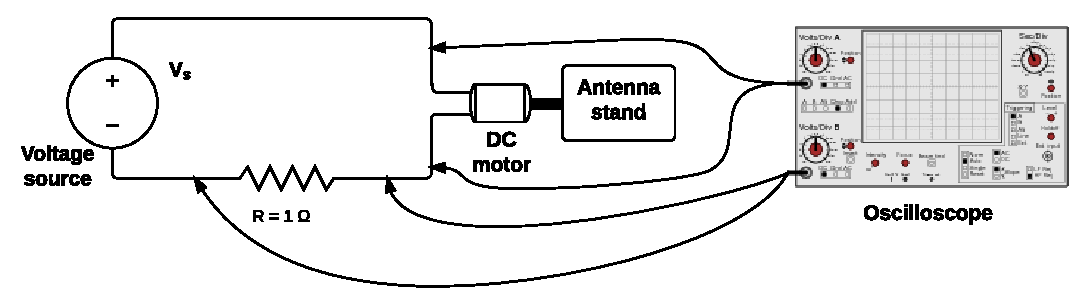
\includegraphics[width=\textwidth]{figures/test/JsCircuit}
        \caption{Diagram of the setup for measuring the moment of inertia. Oscilloscope icon is from \cite{web:OscilloscopeIcon}}
        \label{Appendix:fig:JsSetup}
\end{figure}
\begin{figure} [!h]
    \centering
        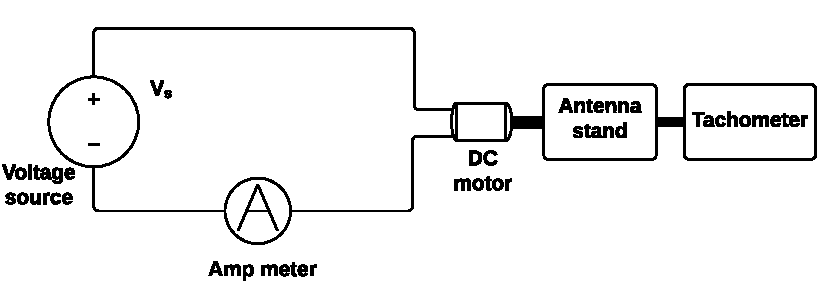
\includegraphics[width=0.8\textwidth]{figures/test/BsCircuit}
        \caption{Diagram of the setup for measuring the friction coefficient.}
        \label{Appendix:fig:BsSetup}
\end{figure}
%$\approx$8 ms for voltage source to rise to 99\% (for 2 to 10 V)

\section*{Method}
The test is done in two parts, one for the friction coefficient and one for the moment of inertia.
\subsection*{Method for friction coefficient}
The motor is connected to a voltage source, in series with an amp-meter. The angular velocity is measured with a tachometer
\begin{enumerate}
\item Apply a voltage with the voltage source.
\item Wait for the system to reach steady state.
\item Measure the current and azimuth angular velocity of the motor stand.
\item Change the voltage and repeat steps 2 to 3.
\end{enumerate}

\subsection*{Method for moment of inertia}
The motor is connected to the resistor and the voltage source. The oscilloscope is connected to the measuring points as indicated on \autoref{Appendix:fig:DCMotorJmSetup}. A voltage step is applied to measure the step response, so a moment of inertia that fits the dynamic properties of the motors rotational body can be determined. A step from \SI{2}{\volt} to \SI{10}{\volt} is applied, since the friction at an angular velocity of $\omega_m = 0$ is expected to be nonlinear. Therefore:
\begin{enumerate}
\item Set the antennas elevation angle to \SI{0}{\degree}.
\item Set the voltage supply to \SI{6}{\volt}.
\item Wait for system to reach steady state.
\item Set the oscilloscope to trigger on the next rising slope.
\item Change the voltage supply to \SI{12}{\volt} in a single step.
\item Save the curve of the voltage and current from the oscilloscope.
\item Repeat steps 2 to 6 with elevation angles \SI{45}{\degree} and \SI{90}{\degree}.
\end{enumerate}

\section*{Results}
The results are split in two, one set for the friction coefficient and one for the moment of inertia.
During testing it is observed that the antenna stand doesn't start rotating before a voltages above $V_{start} = \SI{1.76}{\volt}$ is applied.
\subsection*{Results for friction coefficient}
The results for the friction coefficient are given by \autoref{tab_appendix:testBs}.

\begin{table}[!h]
	\centering
	\caption{Data of the measurement. The angular frequency and friction coefficient are calculated values.}\label{tab_appendix:testBs}
	\begin{tabularx}{\textwidth}{lXXX}
		\gls{rpm} [\si{\per\minute}]& Current, $i_a(t)$ [\si{\milli\ampere}]	& Angular Frequency, $\omega_s(t)$ [\si{\radian\per\second}]& Friction Coefficient, $B_s$ [\si{\newton\metre\second\per\radian}]							\\ \toprule \rowcolor{lightGrey}
		10 & 30,7 & 1,05& 0,039	\\
		13	& 32,4 & 1,36 & 0,028\\ \rowcolor{lightGrey}
		20 & 35,8 & 2,09& 0,015 \\
		25 & 37,2 & 2,62& 0,009 \\ \rowcolor{lightGrey}
		29 & 40,8 & 3,04& 0,007 \\
		36 & 43,6 & 3,77& 0,004\\ 
	\end{tabularx}
\end{table}
\subsection*{Results for moment of inertia}
On \autoref{Appendix:fig:StandMomentOfIntertia} the results from the test are illustrated. The current is calculated by using the voltage across the resistor $R=\SI{1}{\ohm}$ and Ohm's law $V = R \cdot I$.
\begin{figure}[!h]
\centering
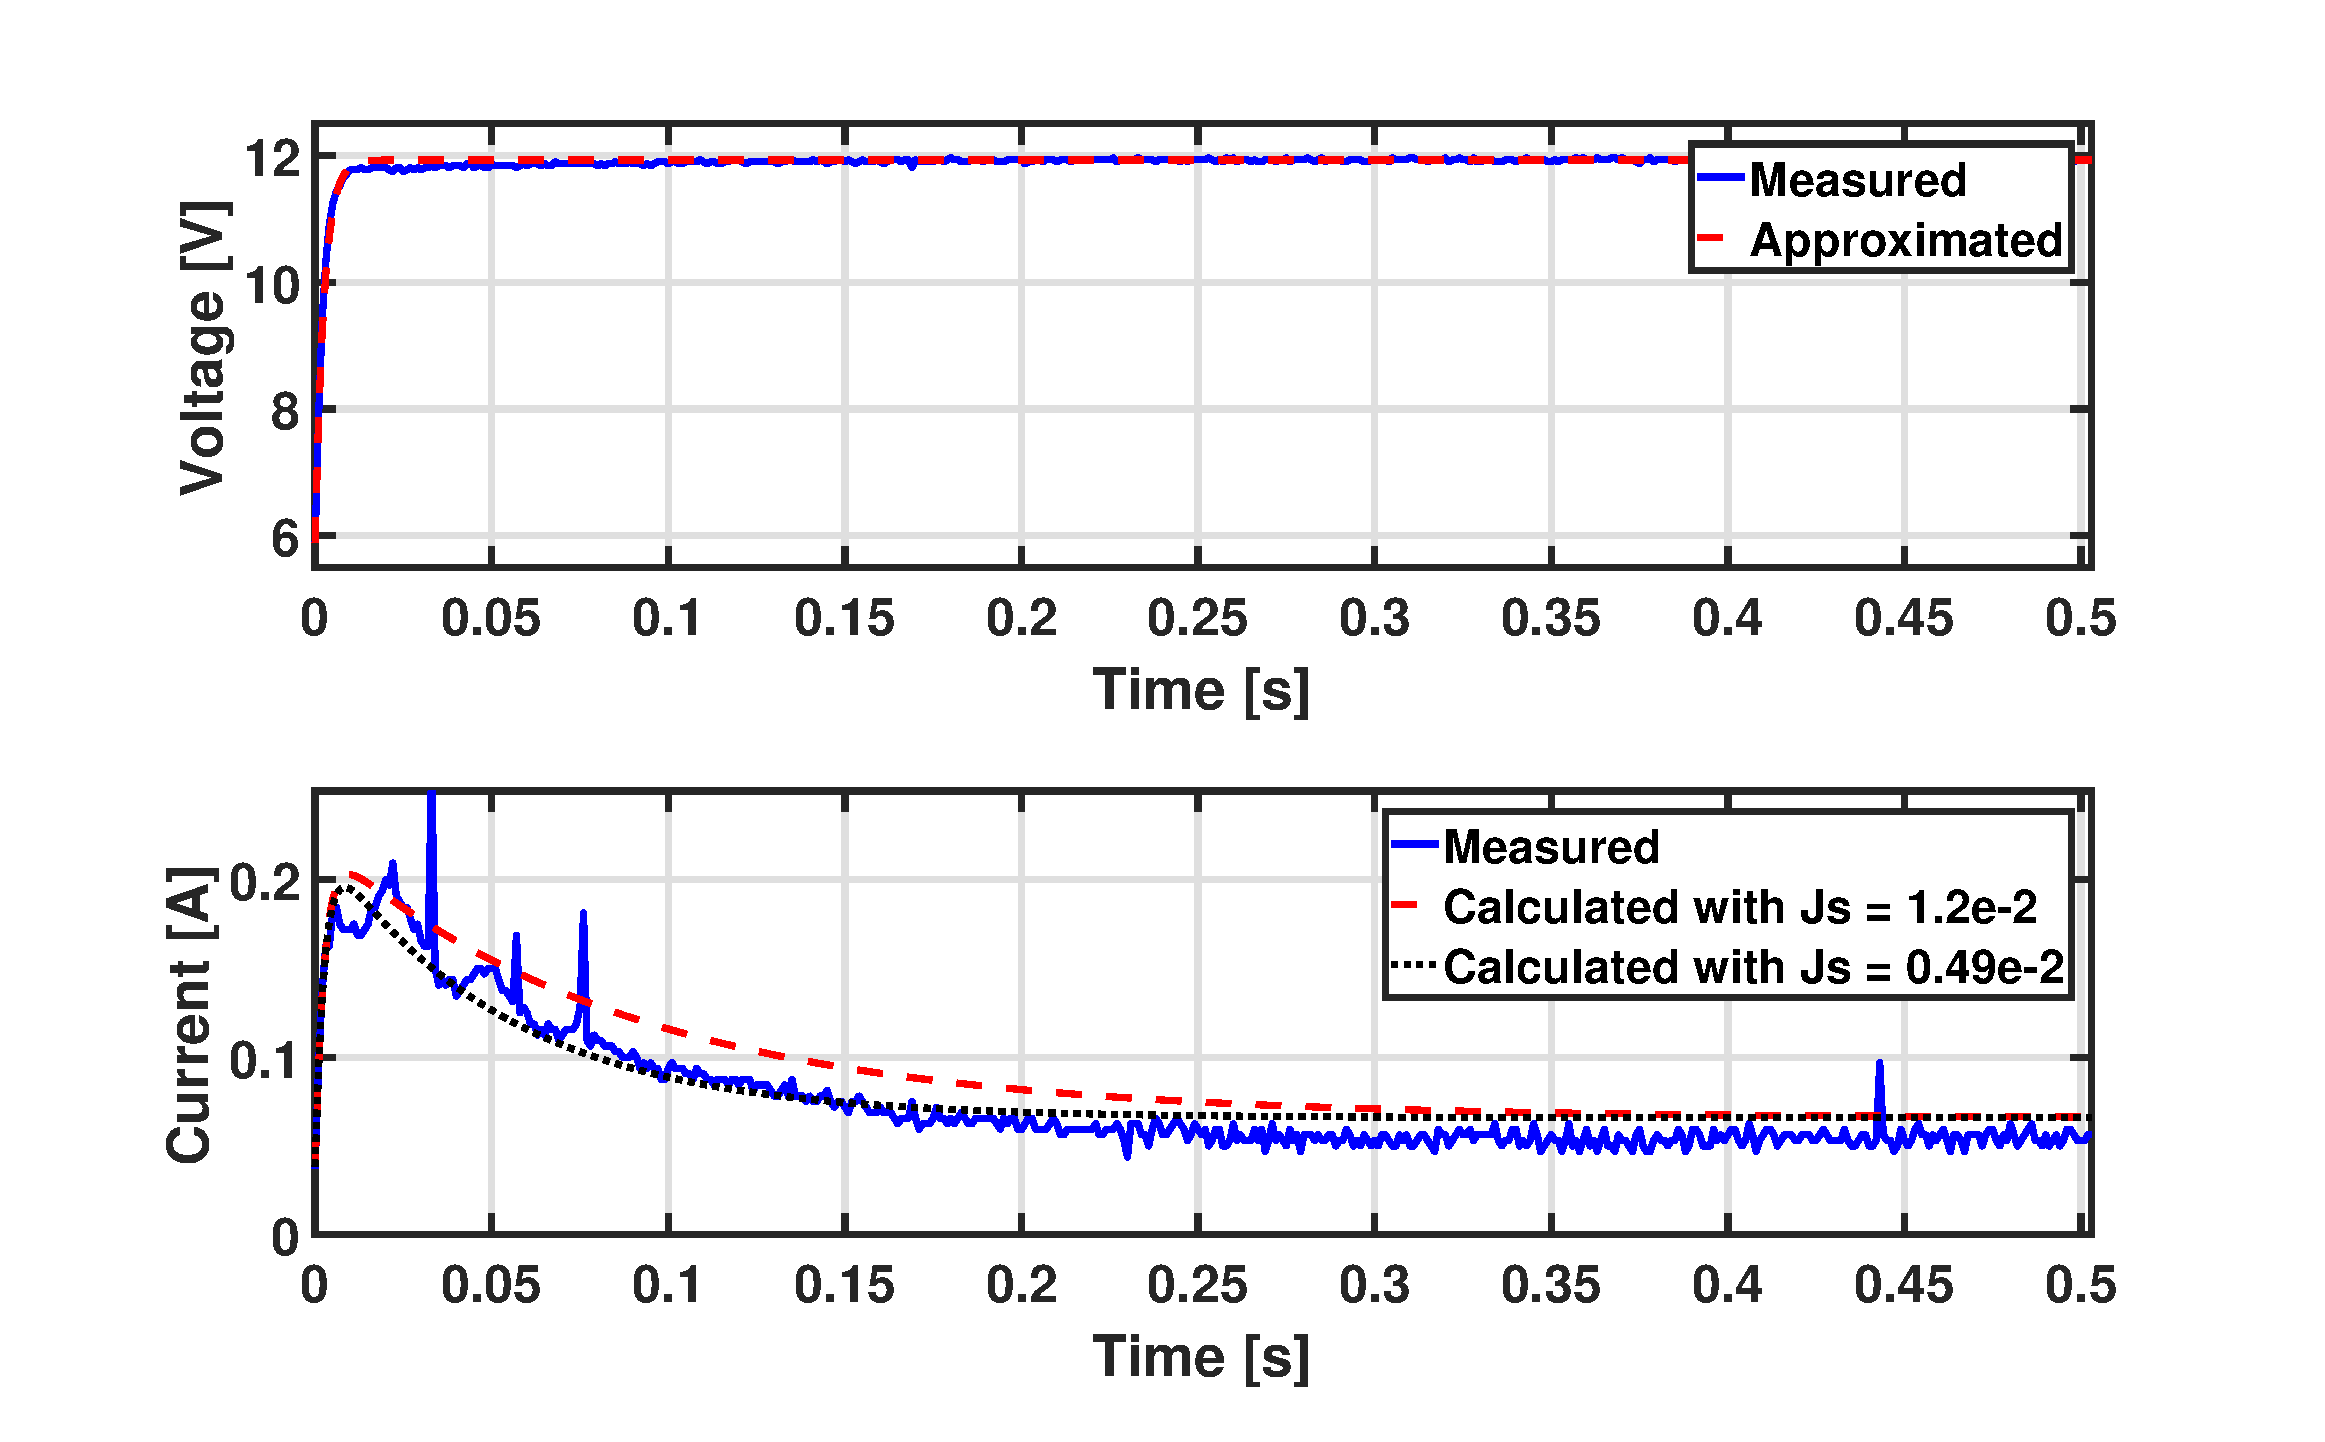
\includegraphics[width=\textwidth]{figures/test/standJsTest}
\caption{A graph of the voltage across the DC motor and the corrosponding current in respect to time. The graph contains the measured and calculated curves.}\label{Appendix:fig:StandMomentOfIntertia}
\end{figure}

\section*{Data processing}
The data processing is also split in two. The friction coefficient $B_s$ is calculated first. Afterwards the moment of inertia $J_s$ is calculated. Before the friction coefficient is calculated, the three differential equations used to describe the model of the motorised antenna stand, Equations \ref{eq:DC-motorElecDone}, \ref{eq:DC-motorMechDone} and \ref{eq:standDiffEquationDone}, from \autoref{sec:standAzimuthModel} is recalled. These equations are given as Equations \ref{appendix:eq:StandDCElec}, \ref{appendix:eq:StandDCMech} and \ref{appendix:eq:StandMech}.
\begin{subequations}
	\begin{align}
	v_{s}(t) = R_{a}\cdot i_a(t) + \frac{d i_a(t)}{d t}\cdot L_a + K_{e}\cdot\omega_{s}(t)\cdot N \addunit{\volt} \label{appendix:eq:StandDCElec}\\ 
	J_m \cdot \frac{d \omega_{s}(t)}{d t}\cdot N = K_t\cdot i_a(t)- \tau_l(t) - B_m \cdot \omega_{s}(t)\cdot N \addunit{\newton\metre} \label{appendix:eq:StandDCMech}\\
	J_s \cdot \frac{d \omega_{s}(t)}{d t} =\tau_l(t) \cdot N - B_s \cdot \omega_{s}(t) \addunit{\newton\metre} \label{appendix:eq:StandMech}
	\end{align}
\end{subequations}

By combining Equations \ref{appendix:eq:StandDCMech} and \ref{appendix:eq:StandMech}, \autoref{appendix:eq:JsStandAzimuthMech} can be determined.%\todo[inline]{Well, that's a strange behaviour, silly latex.}
\begin{equation}
\left(J_m N^2 + J_s\right) \frac{d \omega_{s}(t)}{d t} = K_t i_a(t) N - \left(B_m N^2 + B_s \right)\omega_s(t)  \addunit{\newton\metre\second\per\radian} \phantom{KKKKKKK}\label{appendix:eq:JsStandAzimuthMech}
\end{equation}

\autoref{appendix:eq:JsStandAzimuthMech} is used to calculated the friction coefficient.
\subsection*{Calculation of the friction coefficient}
By analysis of \autoref{appendix:eq:JsStandAzimuthMech} function, it can be seen that if $\omega_s(t)$ is a constant, then the relationship between the current and the friction coefficient is given by \autoref{appendix:eq:StandFriction}.
\begin{equation} 
B_s=\frac{ K_t i_a(t) N}{\omega_s(t)}-B_m N^2\addunit{\newton\metre\second\per\radian} \label{appendix:eq:StandFriction}
\end{equation}

The friction coefficient is determined by calculating the average by \autoref{Appendix:BmCalculationStand}, using the data from \autoref{tab_appendix:testBs}.
\begin{equation}
B_s = \frac{\sum\limits_{n=0}^{x-1} \frac{K_t i_{a}[n] N}{\omega_{s}[n]}-B_m N^2}{x}=\SI{0.017}{\newton\metre\second\per\radian}\label{Appendix:BmCalculationStand}
\end{equation}
\startexplain
\explain{$x$ is the number of measurements}{\noSIunit}
\explain{$n$ is the measurement number from 0 to $(x-1)$}{\noSIunit}
\stopexplain
\subsection*{Calculation of the moment of inertia}
Ideally the voltage curve on \autoref{Appendix:fig:StandMomentOfIntertia} would be a sharp step, and the angular velocity in respect to time would be measured. Since the equipment for such measurements is not available, a measurement of the voltage and current is used. A curve fit between the theoretical model and the measurements is made, so that the model has the same dynamic properties (such as rise time, overshoot and settling time) as the measurements.

By laplace transformation of Equations \ref{appendix:eq:StandDCElec} and \ref{appendix:eq:JsStandAzimuthMech}, Equations \ref{appendix:eq:JsEleclaplace} and \ref{appendix:eq:JsMechlaplace} is derived.
\begin{subequations}
\begin{align} \label{appendix:eq:JsEleclaplace}
V_{s}(s) = R_{a} I_a(s) + \left(I_a(s)  s-i_{init} \right) \cdot L_a + K_{e}\Omega_{s}(s) N      \\
\left(J_m N^2 + J_s\right) \left(\Omega_{s}(s) s - \omega_{sinit}\right) = K_t I_a(s) N - \left(B_m N^2 + B_s \right)\Omega_s(s) \label{appendix:eq:JsMechlaplace}
\end{align}
\end{subequations}

By isolation $\Omega_m(s)$ in \autoref{appendix:eq:JsMechlaplace}, and insert it into \autoref{appendix:eq:JsEleclaplace}, a relationship between the voltage $V_s(s)$ and the current $I_a(s)$ is shown in \autoref{appendix:eq:JsStandTF}.

\begin{equation} \label{appendix:eq:JsStandTF}
I_a(s) =  \frac{ \frac{-K_e N}{L_a}\omega_{sinit}+\frac{(J_m s + B_m) N^2 + J_s s + B_s}{J_m N^2 + J_s} i_{ainit} + \frac{(J_m s + B_m) N^2 + J_s s + B_s}{L_a (J_m N^2 + J_s)} V_s(s)   }{  s^2 + \frac{(B_m N^2 + B_s) L_a + R_a (J_m N^2 + J_s)}{L_a (J_m N^2 + J_s)} s + \frac{B_m N^2 R_a + K_e K_t N^2 + B_s R_a}{L_a (J_m N^2 + J_s)}  } 
\end{equation}

The initial current $i_{init}$ is measured and the initial angular velocity $\omega_{init}$ is calculated using the initial current, initial voltage and \autoref{appendix:eq:StandDCElec}.
The supply voltage $V_s(s)$ is approximated by as an exponential function and applied to the function which is then inverse laplace transformed to describe current in the time domain.
The moment of inertia $J_s$ is then varied to get the best fit of the dynamic properties of the system. All of this is done through MATLAB by the code shown in \autoref{Appendix:lst:DCMotorJsMatlab}.
It is observed that there is a steady state error which might be due to the approximations made in regards to the motor friction coefficient $B_m$ in \autoref{appendix:TJDCMotorTorqueConstant} and the stand's friction coefficient $B_s$.

\lstinputlisting[language = matlab, caption = {Matlab code to approximate the voltage $V_s(s)$ and fit the model of the motorised antenna stand to the measurements}, label = {Appendix:lst:DCMotorJsMatlab}]{appendixCode/momentOfInertiaCurveFitStand.m}
The curve fitting gives a value of $J_s = \SI{0.0049}{\newton\metre\second\squared\per\radian}$, it is however seen that the empirically chosen value $J_s = \SI{0.012}{\newton\metre\second\squared\per\radian}$ has a better fitting rise time, overshoot and settling time compared to the measured data. The value $J_s = \SI{0.012}{\newton\metre\second\squared\per\radian}$ is therefore chosen.

\section*{Conclusion}
The result for the test and calculation is that the moment of inertia of the DC motors rotational body is $J_s = \SI{0.012}{\newton\metre\second\squared\per\radian}$. The friction coefficient is determined to be $B_s =\SI{0.017}{\newton\metre\second\per\radian}$. It should however be noted that this is an approximation, since \autoref{tab_appendix:testBs} shows that the friction coefficient is not constant, as the model otherwise suggests. This approximation will lead to inconsistencies between the model and the real antenna stands properties, such as the DC error seen in \autoref{Appendix:fig:StandMomentOfIntertia}. This error is accepted, since the feedback loop of the whole system should make up for these differences.

It is also noted that the antenna stand does not start rotating before DC voltages above $V_{start} = \SI{1.76}{\volt}$ is applied.